\documentclass[10.5pt,compsoc,twocolumn]{CjC} % 添加 twocolumn 以模拟双栏布局
\usepackage{CJKutf8}
\usepackage{CJK}

\usepackage{subfigure}
\usepackage{url}
\usepackage{multirow}
\usepackage[noadjust]{cite}
\usepackage{amsmath,amsthm}
\usepackage{amssymb,amsfonts}
\usepackage{booktabs}
\usepackage{color}
\usepackage{ccaption}
\usepackage{booktabs}
\usepackage{float}
\usepackage{fancyhdr}
\usepackage{caption}
\usepackage{xcolor,stfloats}
\usepackage{comment}
\setcounter{page}{1}
\usepackage{cuted}%flushend,
\usepackage{captionhack}
\usepackage{epstopdf}
\usepackage{booktabs}
\usepackage{longtable}
\usepackage{array}
\usepackage{amsmath}
\usepackage{xeCJK}
\usepackage{listings}
\usepackage{xcolor}
\usepackage{array}
\usepackage{CJKutf8}

\usepackage{tabularx}



\usepackage{caption}


\usepackage{float} % 用于 [H] 强制定位
% 定义代码风格

\usepackage{longtable}

%\usepackage{ccmap}
%\CJKtilde
%\usepackage{CJKpunct} 
%\usepackage[lite,subscriptcorrection,slantedGreek,nofontinfo]{mtpro2}

%===============================%

% \firstfootname{ \quad \quad }
\headevenname{\mbox{\quad} \hfill  \mbox{\zihao{-5}{\begin{CJK*}{UTF8}{song}数据库原理与应用\end{CJK*}} \hspace {50mm} \mbox{\begin{CJK*}{UTF8}{song}2026 年\end{CJK*}}}}%
\headoddname{\begin{CJK*}{UTF8}{song}\hfill
Awesql:一种集成自然语言查询与SQL智能校验的数据库命令行工具\end{CJK*}}%

%footnote use of *
\renewcommand{\thefootnote}{\fnsymbol{footnote}}
\setcounter{footnote}{0}

\newtheoremstyle{mystyle}{0pt}{0pt}{\normalfont}{1em}{\bf}{}{1em}{}
\theoremstyle{mystyle}
\renewcommand{\thesubfigure}{(\alph{subfigure})}
\newcommand{\upcite}[1]{\textsuperscript{\cite{#1}}}
\renewcommand{\labelenumi}{(\arabic{enumi})}
\newcommand{\tabincell}[2]{\begin{tabular}{@{}#1@{}}#2\end{tabular}}
\newcommand{\abc}{\color{white}\vrule width 2pt}
\makeatletter
\renewcommand{\@biblabel}[1]{[#1]\hfill}
\makeatother
\setlength\parindent{2em}
% \renewcommand{\hth}{\begin{CJK*}{UTF8}{zhhei}}
% \renewcommand{\htss}{\begin{CJK*}{UTF8}{song}}

\input{zhwinfonts}

\hyphenpenalty=50000
\makeatletter
\newcommand\mysmall{\@setfontsize\mysmall{7}{9.5}}
\newenvironment{tablehere}
  {\def\@captype{table}}

\let\temp\footnote
\renewcommand \footnote[1]{\temp{\zihao{-5}#1}}


\thispagestyle{plain}%
\thispagestyle{empty}%
\pagestyle{CjCheadings}

\begin{document}
\begin{table*}[!t]
\vspace {-13mm}
\begin{tabular}{p{168mm}}
\zihao{5-}\begin{CJK*}{UTF8}{song}
2025年6月 \hfill数据库原理与应用\end{CJK*}\\
\hline\\[-4.5mm]
\hline\end{tabular}

\centering
\vspace {11mm}
\begin{CJK*}{UTF8}{zhhei}
{\zihao{2}Awesql:一种集成自然语言查询与SQL智能校验的数据库命令行工具}
\end{CJK*}
\vskip 5mm

{\zihao{3}\begin{CJK*}{UTF8}{fs}
和嘉炜\quad  韩璐帆 \quad 鄢怡然\end{CJK*}}

\vspace {5mm}
\zihao{6}{\begin{CJK*}{UTF8}{song}
西南财经大学\quad统计与数据科学学院\quad数据科学与大数据技术
\end{CJK*}}

\vskip 5mm
{\centering
\begin{tabular}{p{160mm}}
\zihao{5-}{
\setlength{\baselineskip}{16pt}\selectfont{
\noindent\begin{CJK*}{UTF8}{zhhei}摘\quad 要\quad \end{CJK*} \begin{CJK*}{UTF8}{song}
本文设计并实现了一个基于现代命令行交互框架的数据库命令行工具,结合数据库管理技术与自然语言处理方法,旨在提升数据库操作的便捷性与智能化水平。系统围绕数据库初始化与关系模式录入、SQL语句智能检查、自然语言查询以及查询流程与结果可视化四大核心功能模块展开。用户可通过命令行快速完成数据库的创建、表结构定义及数据录入,并可重置数据库结构与数据。系统内置SQL语法分析与异常捕捉机制,能够实时识别并反馈查询语句中的语法或逻辑错误,并提供友好的中文报错与修正建议。此外,系统集成Text2SQL转译功能,实现自然语言到SQL语句的自动转换,降低非专业用户的使用门槛。针对复杂查询,系统提供查询执行流程可视化功能,直观展示数据流动路径,同时配备多种图形化结果展示形式,提升数据分析与解读效率。实验表明,该系统具备良好的交互性、扩展性与实用价值,适用于多种轻量级数据管理场景。我们的工具开源在 \url{https://github.com/Hepisces/db_final}。

\end{CJK*}\par}}\\[2mm]

\zihao{5-}{\noindent
\begin{CJK*}{UTF8}{zhhei}关键词\end{CJK*} \quad \begin{CJK*}{UTF8}{song}{数据库命令行工具;SQL语句检查;Text2SQL;自然语言查询;数据可视化}
\end{CJK*}
}\\[2mm]
\vskip 7mm

\end{tabular}}
\begin{center}
\zihao{3}{ {\begin{CJK*}{UTF8}{zhhei}Awesql: A Database Command Line Tool Integrating Natural Language Querying and SQL Intelligent Checking\end{CJK*}}}\\
\vspace {5mm}
\zihao{5}{ {\begin{CJK*}{UTF8}{zhhei}Jiawei He Lufan Han Yiran Yan \end{CJK*}
}}\\
\vspace {2mm}
\zihao{6}{\begin{CJK*}{UTF8}{zhhei}{Southwestern University of Finance and Economics\quad School of Statistics and Data Science\quad Data Science and Big Data Technology }\end{CJK*}}

\end{center}
\begin{tabular}{p{160mm}}
\zihao{5}{
\setlength{\baselineskip}{18pt}\selectfont{
{\bf Abstract}\quad \par}}\setlength{\baselineskip}{18pt}\selectfont{\zihao{5}{\noindent This paper designs and implements a database command line tool based on a modern command line interaction framework, which combines database management techniques and natural language processing methods, aiming to improve the convenience and intelligence of database operation. The system revolves around four core functional modules: database initialization and relational schema entry, SQL statement intelligent checking, natural language query, and query process and result visualization. Users can quickly complete database creation, table structure definition and data entry through the command line, and can reset the database structure and data. The system has a built-in SQL syntax analysis and anomaly capture mechanism, which can identify and feedback syntax or logic errors in query statements in real time, and provide friendly Chinese error reporting and correction suggestions. In addition, the system integrates Text2SQL translation function, which realizes automatic conversion from natural language to SQL statement and reduces the threshold for non-professional users. For complex queries, the system provides query execution process visualization function, which intuitively displays the data flow path, and is equipped with multiple graphical results display forms to enhance the efficiency of data analysis and interpretation. Experiments show that the system has good interactivity, scalability and practical value, and is suitable for a variety of lightweight data management scenarios. Our tools are open source at \url{https://github.com/Hepisces/db_final}.

\vspace {5mm}
{\bf Keywords}\quad \begin{CJK*}{UTF8}{zhhei}
{Database Command Line Tools; SQL Statement Checking; Text2SQL; Natural Language Queries; Data Visualization}
\end{CJK*}}\par}
\end{tabular}
\end{table*}
\vskip -3mm
\clearpage

{\begin{CJK*}{UTF8}{zhhei}\zihao{5}\vskip 1mm\section{引言}\end{CJK*}}
{\begin{CJK*}{UTF8}{zhhei}\vskip 1mm\subsection{研究背景与意义}\end{CJK*}}
\begin{CJK*}{UTF8}{song}
随着信息技术的迅猛发展和数据规模的持续扩大,数据库及数据库管理系统(Database Management System, DBMS)已成为现代信息系统不可或缺的核心组件。数据库技术广泛应用于金融、电商、医疗、政务、科研、司法等诸多领域,承担着数据存储、管理、查询与分析的重要职责。数据库技术能方便地维护数据、更严密地控制数据和更有效地利用数据,数据库的数据存储具有冗余度小、易共享和独立性强等特点[1]。

关系型数据库管理系统(Relational Database Management System, RDBMS)凭借其成熟的事务管理机制、灵活的结构化查询语言SQL(Structured Query Language, SQL)以及良好的数据一致性保障,成为目前应用最为广泛的数据库类型之一。关系型数据库是以多个表格的形式进行表达,并将数据存储在表格中的数据库系统[2],每个表格以每一组行和列的数据组成。关系型数据库遵循结构化查询语言的标准,使用SQL来执行数据的增删和改查的操作,SQL作为一种强大的查询语言,它使得用户能够灵活地查询、增加、更新和删除数据。关系型数据库的优点在于数据结构非常清晰,容易理解且易于维护,具有事务一致性。这样的优势让它适用于需要严格保证数据完整性的应用场景。

数据库发展迅速并被广泛应用的当下,对于需要快速上手的非专业用户,数据库的使用仍存在一定的门槛。首先,数据库环境的搭建与配置通常较为繁琐,对于非专业用户而言存在技术障碍。其次,关系型数据库依赖SQL语言进行数据操作与查询,尽管SQL是一种声明式语言,即关注于实现目的而非实现过程,但快速学习与掌握SQL语法规则、查询流程、优化手段对于初学者同样存在学习成本。此外,不管是命令行窗口还是数据库管理工具,其都缺乏可视化直观反馈,体现在:查询流程往往隐藏于后台,用户难以及时理解查询逻辑及数据流动路径,不利于排查问题与优化查询;执行结果往往以表格形式展示,难以直观表达数据蕴含的丰富信息。

为此,本研究专注于设计一种集成化、智能化、交互友好、可视化的数据库命令行工具,具备数据库快速初始化、关系模式便捷录入、SQL语句智能纠错、自然语言查询、查询流程与结果可视化等功能,将极大降低数据库应用门槛,提升数据交互效率和使用体验,具有重要的理论价值与实践意义。

\end{CJK*}
{\begin{CJK*}{UTF8}{zhhei}\vskip 1mm\subsection{研究内容}\end{CJK*}}
\begin{CJK*}{UTF8}{song}

本文设计并实现了一个数据库命令行工具,该工具基于现代命令行交互框架,结合数据库管理技术与自然语言处理方法,围绕以下几个核心功能模块展开:

(1)便捷实现数据库初始化与关系模式录入

用户可直接通过命令行快速创建数据库,输入预设的数据库定义语言(data-definition language, DDL),录入关系模式,完成表结构设计与数据录入工作,简化了传统图形界面数据库软件的安装与配置过程。同时本系统设计了数据库结构与数据重置功能,用户可快速清除现有数据库,重新录入关系模式与数据,保障系统使用的灵活性和可扩展性,便于系统推广与使用。

(2)SQL语句智能检查

针对用户输入的SQL查询语句,系统通过外接大模型,内置了语法分析与异常捕捉机制,能够实时检测查询语句中的语法错误、逻辑错误或语义不规范,返回用户友好的中文报错信息,并给出合理的修改建议。例如,当发现字段名拼写错误、缺失关键字或逻辑错误时,系统可指出具体错误位置和可能的修正方式,极大降低用户因语法生疏导致的查询失败率。

(3)自然语言查询

系统加入Text2SQL的转译功能,用户可直接通过自然语言输入查询意图,系统调用自然语言处理模块,加载Text2SQL的转译模型,将其转换为合法SQL语句并执行。如果用户需要确认准确性,可以再次进行SQL语句智能检查。此功能进一步降低非专业用户操作数据库的学习成本,提升交互便捷性。

(4)查询流程与结果可视化

系统可以返回查询执行流程,清晰展示表连接顺序、筛选条件、生成功能列等数据流动路径,帮助用户直观理解复杂查询的内部执行逻辑。同时,对于查询结果,本文也设计了交互功能,用户可以自主选择想要直观分析的属性,以及属性间生成的图形形式,系统设置了时间序列折线图、成对散点图、堆叠柱状图等多种图形,能够提升结果解读效率,方便用户核验与后续处理。

\end{CJK*}
{\begin{CJK*}{UTF8}{zhhei}\vskip 1mm\subsection{文章结构}\end{CJK*}}
\begin{CJK*}{UTF8}{song}

本文的文章设计结构如下:
第二节从基础原理上介绍了组成该命令行工具各个模块使用的“相关技术与方法基础”;
第三节介绍了实验时所使用的智能家居数据库的逻辑设计;
第四节介绍了整体系统设计与各个功能板块的设计;
第五节展示了命令行工具的功能测试与效果;
第六节对本研究工作进行了全面的总结与展望。

\end{CJK*}
{\begin{CJK*}{UTF8}{zhhei}\zihao{5}\vskip 1mm\section{相关技术与方法基础}\end{CJK*}}
{\begin{CJK*}{UTF8}{zhhei}\subsection{Text2SQL模型原理}\end{CJK*}}
\begin{CJK*}{UTF8}{song}

Text2SQL 技术旨在将自然语言查询转化为 SQL 语句,以高效访问关系型数据库。传统方法依赖深度学习和预训练模型,但在语义理解、复杂查询及跨域泛化上存在局限性~\cite{3}。2023 年后,大语言模型(LLM)驱动的方法占据主流,分为四类:Prompt、Fine-tuning、Agent 和混合方法~\cite{7,8,9}。本文所使用的Text2sql模型为在huggingface开源的sqlcoder-7b模型 \footnote{https://huggingface.co/defog/sqlcoder-7b-2}。该模型在CodeLlama-7B~\cite{10}上微调得到,并通过SQL\_Eval进行测试和调整性能,并在date,group\_by,order\_by, ratio, join, where六个类别的生成任务上达到了平均超过90\%的准确率。在使用时,通过传入自然语言查询和目标数据库的关系模式,模型即可返回对应的查询语句。

\end{CJK*}
{\begin{CJK*}{UTF8}{zhhei}\vskip 1mm\subsection{SQL验证}\end{CJK*}}
\begin{CJK*}{UTF8}{song}


SQL验证的早期形式是语法检查,解决语法及词法层面的错误。这一时期的数据库管理系统侧重于管理持久数据,验证较为初级,不涉及运行时语义理解,主要与语法有关,如关键字拼写错误、括号不平衡或运算符位置不正确等问题。为实现对这类错误的自动化检测,业界普遍采用基于上下文无关文法(CFG)的解析器生成工具(Yacc/Bison, ANTLR)来构建抽象语法树,并通过启发式算法来修正拼写错误。

随着SQL成为标准查询语言,应用范围越来越广大,SQL的验证机制也得到了更强的提升,逐步从语法检查过渡到语义分析。语义检查的核心在于验证查询与数据库Schema的一致性,验证对数据库对象的引用是否有效,以及数据类型是否正确,从而解决语法以外的问题。在数据库Oracle的使用文档中就使用了预编译器中的SQLCHECK选项强调了这种转换——该选项允许用户控制检查的范围,可以设置为SYNTAX进行基本语法验证,也可以设置为SEMANTICS进行语法和语义检查。

随着深度学习技术的落地应用和交叉兴起,更多的研究者选择开发专门的深度学习模型来理解SQL查询的语义并生成获修正查询,text2sql任务成为核心,数据集WikiSQL、Spider等数据集为各种模型提供了基准测试,极大地推动了相关模型的发展。在工程实践层面,SQL验证也开始被深度集成到现代软件开发的持续集成/持续部署管道中,通过自动化的静态代码分析和测试,确保任何进入代码库的查询都经过了可靠性验证,保障了生产环境的稳定性。

当前,SQL验证已进入由大语言模型驱动的AI辅助时代,利用LLM的少样本推理能力和上下文机制构建灵活的SQL纠错与优化系统已不鲜见。另外,超越了传统作为文本或代码生成器的角色,LLM驱动的Agent正被验证为一种强大的通用问题解决工具,能够自主执行复杂的多步骤任务。一个功能完备的自主Agent系统,其核心是在LLM强大的推理能力之上,构建了三个相辅相成的关键组件:规划(Planning)、记忆(Memory)和工具使用(Tool Use)。基于LLM Agent的框架,可将SQL验证视为一个由推理和行动组成的动态过程,Agent能够根据用户给出的复杂任务和指令,自主规划验证步骤、调用外部工具,展现出超高的任务适配性和纠错能力。


SQL的验证过程也因此变得更加便捷和具有交互性,一些AI辅助工具如AI2SQL、SQLAI.ai等不仅可以验证语法和语义,还能建议性能优化。这些工具往往支持跨多种数据库方言的验证,并通过自然语言对话帮助用户理解错误根源和优化方案,提升了开发与数据分析的效率。至此,SQL验证已从早期单纯追求语法层面的正确性,演化为一个追求任务适配、执行效率和人机协同的综合智能任务。


\end{CJK*}
{\begin{CJK*}{UTF8}{zhhei}\vskip 1mm\subsection{SQL查询流程与执行原理}\end{CJK*}}
\begin{CJK*}{UTF8}{song}
这部分的核心目的是将不直观的查询执行变为人类易于理解的树状结构流程。现有的多数关系型数据库如PostgreSQL,SQLite等都内置了EXPLAIN QUERY PLAN的功能,这个命令可以输出一个结构化的表格,描述数据库引擎为响应一个SQL查询而将执行的一系列底层操作,通过这个功能即可快速得到数据库的查询计划。由于查询流程本质上是一个有向无环图,但是通过EXPLAIN QUERY PLAN将每个操作赋予唯一ID后可以将图简化为树状结构,此时通过从根结点开始遍历每一个操作节点,即可迭代构建为一个完整的执行树,并在控制台输出。

\end{CJK*}
{\begin{CJK*}{UTF8}{zhhei}\vskip 1mm\subsection{SQL查询流程与查询结果可视化方法}\end{CJK*}}
\begin{CJK*}{UTF8}{song}

对查询结果的可视化分为表格化呈现和图形化呈现两个部分,表格化呈现即直观返回数据库查询结果,图形化的呈现则加入了操作者的先验信息,通过操作者自助判断表格数据类型,再经由可交互命令行做合法性判断,即可返回图形结果如柱状图,点状图等,提供视觉效果更强的数据透视。
\end{CJK*}
{\begin{CJK*}{UTF8}{zhhei}\zihao{5}\vskip 1mm\section{数据库关系模式设计}\end{CJK*}}
\begin{CJK*}{UTF8}{song}

\begin{CJK*}{UTF8}{song}

本研究数据集来自iFLYTEK AI开发者大赛——“智能家居使用场景识别挑战赛”,比赛提供4类数据:账号信息、设备列表、控制操作日志、设备上报日志。数据集分为两个部分,第一部分数据有使用场景标签,第二部分不包含场景标签,由于本研究不涉及场景区分,全部纳入数据库建设中。

{\begin{CJK*}{UTF8}{zhhei}\vskip 1mm\subsection{智能家居E-R图}\end{CJK*}}
E-R模型图是实体-联系图(Entity Relationship Diagram)的简称,它提供了实体、属性和联系的表示方法,是用来描述现实世界的概念模型。在进行智能家居系统数据库设计时,首先需要设计智能家居E-R图。根据比赛提供的数据集,本研究分别建立了家居账号信息(customer)、账号设备列表(devList)、控制操作日志(control)、设备上传日志(devUpdata)四个实体集,实体集通过联系集相互关联的模式如下图所示:
\begin{figure}[H] % 强制图片紧跟文字下方
  \raggedright % 强制靠左对齐
  \makebox[0pt][l]{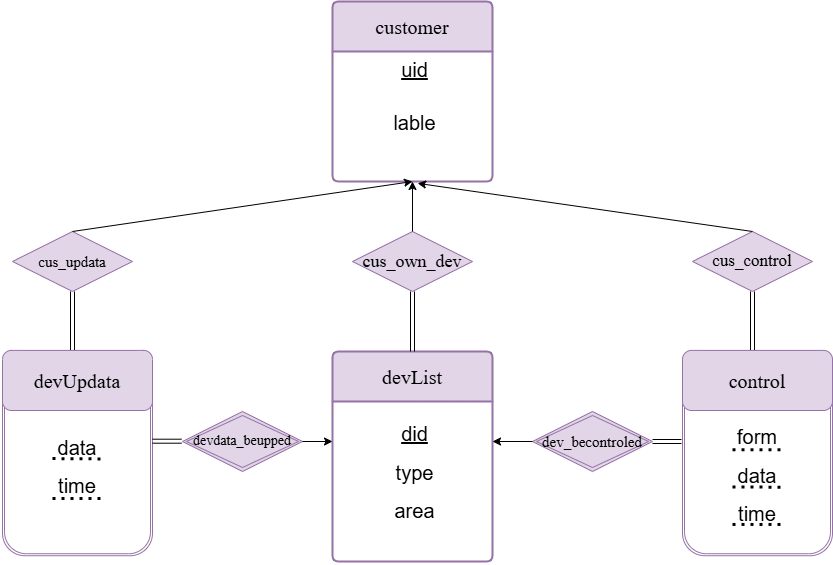
\includegraphics[width=0.48\textwidth]{article/design/figures/smart_home_ER.png}} % 靠左,限制宽度
  \caption{智能家居E-R图}
  \label{fig:smart_home_ER}
\end{figure}

{\begin{CJK*}{UTF8}{zhhei}\subsection{智能家居数据库逻辑设计}\end{CJK*}}

数据库逻辑设计是指在设计数据库结构时,定义表、列、关系和约束等元素的过程。它的目标是根据应用程序需求和数据关系,合理地组织和规划数据库的结构,以实现数据的有效存储、检索和管理。根据上文的智能家居E-R图,将E-R图转化为关系模式,各表的表结构如下:

\begin{enumerate}

    \item 基本信息表:
    
基本信息表也可称为静态信息类表,用于保存智能家居系统中家庭账户信息,智能家居设备信息。基本信息共有两张表:家居账号信息表(customer)与账号设备列表(devList),如下表所示:
    \begin{table}[H]
    \centering
    \caption{家居账号信息表(customer)}
    \vspace{2mm}
    \small
    \begin{tabular}{lllllp{2cm}}
    \toprule
        \textbf{属性} & \textbf{数据类型} & \textbf{长度} & \textbf{主键} & \textbf{外键} & \textbf{含义解释} \\
        \hline
        uid & VARCHAR & 35 & Y & N & 账号id,唯一标识一个账号 \\
        label & INTEGER & 1 & N & N & 使用场景 \\
        \bottomrule
    \end{tabular}
    \label{tab1}
    \end{table}
    \begin{table}[H]
    \centering
    \caption{账号设备列表(devList)}
    \vspace{2mm}
    \small
    \begin{tabular}{lllllp{2cm}}
    \toprule
        \textbf{属性} & \textbf{数据类型} & \textbf{长度} & \textbf{主键} & \textbf{外键} & \textbf{含义解释} \\
        \hline
        uid & VARCHAR & 35 & N & Y & 账号id,唯一标识一个账号 \\
        did & VARCHAR & 35 & Y & N & 设备id \\
        type & VARCHAR & 4 & N & N & 设备型号 \\
        area & VARCHAR & 20 & N & N & 设备房间标签 \\
        \bottomrule
    \end{tabular}
    \label{tab1}
    \end{table}
    \item 实时动态信息表:
    
动态信息表用于记录智能家居中账户对各种家电智能设备的操控监测数据以及设备状态上传信息。实时动态信息一共有两张表:控制操作日志(control)、设备上传日志(devUpdata),如下表所示:
    \begin{table}[H]
    \centering
    \caption{控制操作日志(control)}
    \vspace{2mm}
    \small
    \begin{tabular}{lllllp{2cm}}
    \toprule
        \textbf{属性} & \textbf{数据类型} & \textbf{长度} & \textbf{主键} & \textbf{外键} & \textbf{含义解释} \\
        \hline
        uid & VARCHAR & 35 & N & Y & 账号id,唯一标识一个账号 \\
        did & VARCHAR & 35 & Y & Y & 控制的设备id \\
        time & TIMESTAMP & 20 & Y & N & 控制时间 \\
        form & VARCHAR & 15 & Y & N & 控制方式 \\
        data & VARCHAR & 20 & Y & N & 从远程对设备下发的控制日志 \\
        \bottomrule
    \end{tabular}
    \label{tab1}
    \end{table}
    \begin{table}[H]
    \centering
    \caption{设备上传日志(devUpdata)}
    \vspace{2mm}
    \small
    \begin{tabular}{lllllp{2cm}}
    \toprule
        \textbf{属性} & \textbf{数据类型} & \textbf{长度} & \textbf{主键} & \textbf{外键} & \textbf{含义解释} \\
        \hline
        uid & VARCHAR & 35 & N & Y & 账号id,唯一标识一个账号 \\
        did & VARCHAR & 35 & Y & Y & 上报的设备id \\
        time & TIMESTAMP & 20 & Y & N & 上报时间 \\
        data & VARCHAR & 20 & Y & N & 设备上报的状态日志 \\
        \bottomrule
    \end{tabular}
    \label{tab1}
    \end{table}


\end{enumerate}
\end{CJK*}



\end{CJK*}
{\begin{CJK*}{UTF8}{zhhei}\zihao{5}\vskip 1mm\section{系统设计}\end{CJK*}}
\begin{CJK*}{UTF8}{song}


\end{CJK*}
{\begin{CJK*}{UTF8}{zhhei}\subsection{系统架构设计}\end{CJK*}}
\begin{CJK*}{UTF8}{song}

我们设计的命令行工具采用分层架构, 将功能按逻辑划分为三个主要层:表现层、业务逻辑层和数据访问层,每一层通过不同的组件实现。

{\begin{CJK*}{UTF8}{zhhei}\subsubsection{表现层}\end{CJK*}}

表现层通过cli.py实现,作为唯一入口,负责与用户直接交互。这一层通过typer和rich库完成命令行的交互式,可以通过解析用户输入的命令(如 init, ask, run, reset)和参数,调用对应实现逻辑,并将最终结果(文本、表格、图表路径)格式化后呈现给用户。
{\begin{CJK*}{UTF8}{zhhei}\subsubsection{业务逻辑层}\end{CJK*}}

业务逻辑层通过 Text2SQL.py, checker.py, visualizer.py 分别实现,处理所有核心任务。Text2SQL.py可以将用户的自然语言问题转换为结构化查询语言(SQL),并结合数据库关系模式作为提示词与LLM进行交互。checker.py 模块作为一个关键的验证器,负责对用户输入或AI生成的SQL查询进行语法和基础语义的合法性检查,确保执行的查询是安全和有效的。visualizer.py 模块负责所有可视化任务,将抽象的查询计划(Query Plan)和查询结果(Result Set)数据,分别转换为人类易于理解的树状图和多种统计图表(如柱状图、折线图等)。

{\begin{CJK*}{UTF8}{zhhei}\subsubsection{数据访问层}\end{CJK*}}

数据访问层通过db.py 实现,封装了所有与底层数据库SQLite的交互细节,所有上层模块都通过此层访问数据库,实现包括但不仅限于数据库连接、表结构创建(DDL执行)、数据导入、查询执行(包括 \textit{EXPLAIN QUERY PLAN})以及数据库重置等功能。
值得一提的是,无论是从数据库获取的查询结果,还是查询计划,都被统一抽象为DataFrame。这可以极大地简化在不同模块(如 db, checker, visualizer)之间的数据传递和处理流程。

\end{CJK*}
{\begin{CJK*}{UTF8}{zhhei}\vskip 1mm\subsection{功能模块设计}\end{CJK*}}

{\begin{CJK*}{UTF8}{zhhei}\subsubsection{数据库初始化}\end{CJK*}}
\begin{CJK*}{UTF8}{song}

此模块负责为首次运行系统准备必要的数据库环境。用户在命令行执行 \textit{awesql import-data} 命令,该命令有两个可选参数,分别为\textit{--der}和\textit{—db-name},分别指定数据文件夹路径和数据库名称,默认参数分别为Smart\_Home\_DATA 和project2025。

命令输入后,系统首先调用 db.db\_exists() 检查预定义的数据库文件(如 project2025.db)是否存在且包含数据。若已存在,则提示用户并终止操作,防止意外覆盖;若数据库不存在,系统会查找指定数据目录下的 DDL.sql 文件,通过 db.create\_tables() 函数,读取该文件内容并利用 sqlite3 的 executescript() 方法一次性执行所有 CREATE TABLE 语句,完成数据库表结构的构建。

表结构创建成功后, 系统通过 db. import\_real\_data() 函数,按预设的并且符合外键依赖关系的顺序(例如$ customer.sql \rightarrow devlist.sql \rightarrow ...$),逐一读取数据目录下的 .sql 文件。对每个文件中的每一行 INSERT 语句进行处理和执行,将数据填充到相应的表中。

同时,为了后续操作的需要,在首次初始化时,db.create\_default\_config\_if\_not\_exists() 会自动创建 awesql\_config.json 配置文件,并将 DDL.sql 的路径记录其中,供后续模块(如Text2SQL)使用。

为了设计简便,系统强制要求创建表结构的文件命名为DDL.sql,并与所有导入数据的文件存放在同一文件夹,导入数据文件的名称也需要与表名称一致。


\end{CJK*}
{\begin{CJK*}{UTF8}{zhhei}\subsubsection{SQL正确性检查与建议}\end{CJK*}}
\begin{CJK*}{UTF8}{song}

在实际业务开发中,SQL作为数据库交互的主要手段,其正确性直接影响数据处理与系统运行的可靠性。然而,大多数SQL校验工具都局限于基础的语法层和语义层面检查,对于代码本身的性能隐患以及代码规范性等深层的问题缺乏关注,在实际应用中存在不足,从而影响系统性能与维护性。并且,此类工具提供的修正建议通常较为泛化,在用户体验上尚有不足,尤其对于初级开发者而言,难以高效地定位问题本质,获得有效的优化指导。

为改善这些问题,我们设计并实现了一个新颖的SQL验证模块,即4.1节提到的SQL checker。这个模块是由大语言模型Deepseek驱动、加入上下文注入与思维链引导的Agent,可以实现对SQL语句进行深度分析,提供覆盖语义正确性、性能优化及代码规范三方面的综合性建议。

\textbf{(1)工作流}

工作流的最终产出,是一份包含语法语义结构检查、并结合性能与上下文考量的综合性分析报告。其工作流示意图如Fig.~\ref{fig:agent}所示。


\begin{figure*}
  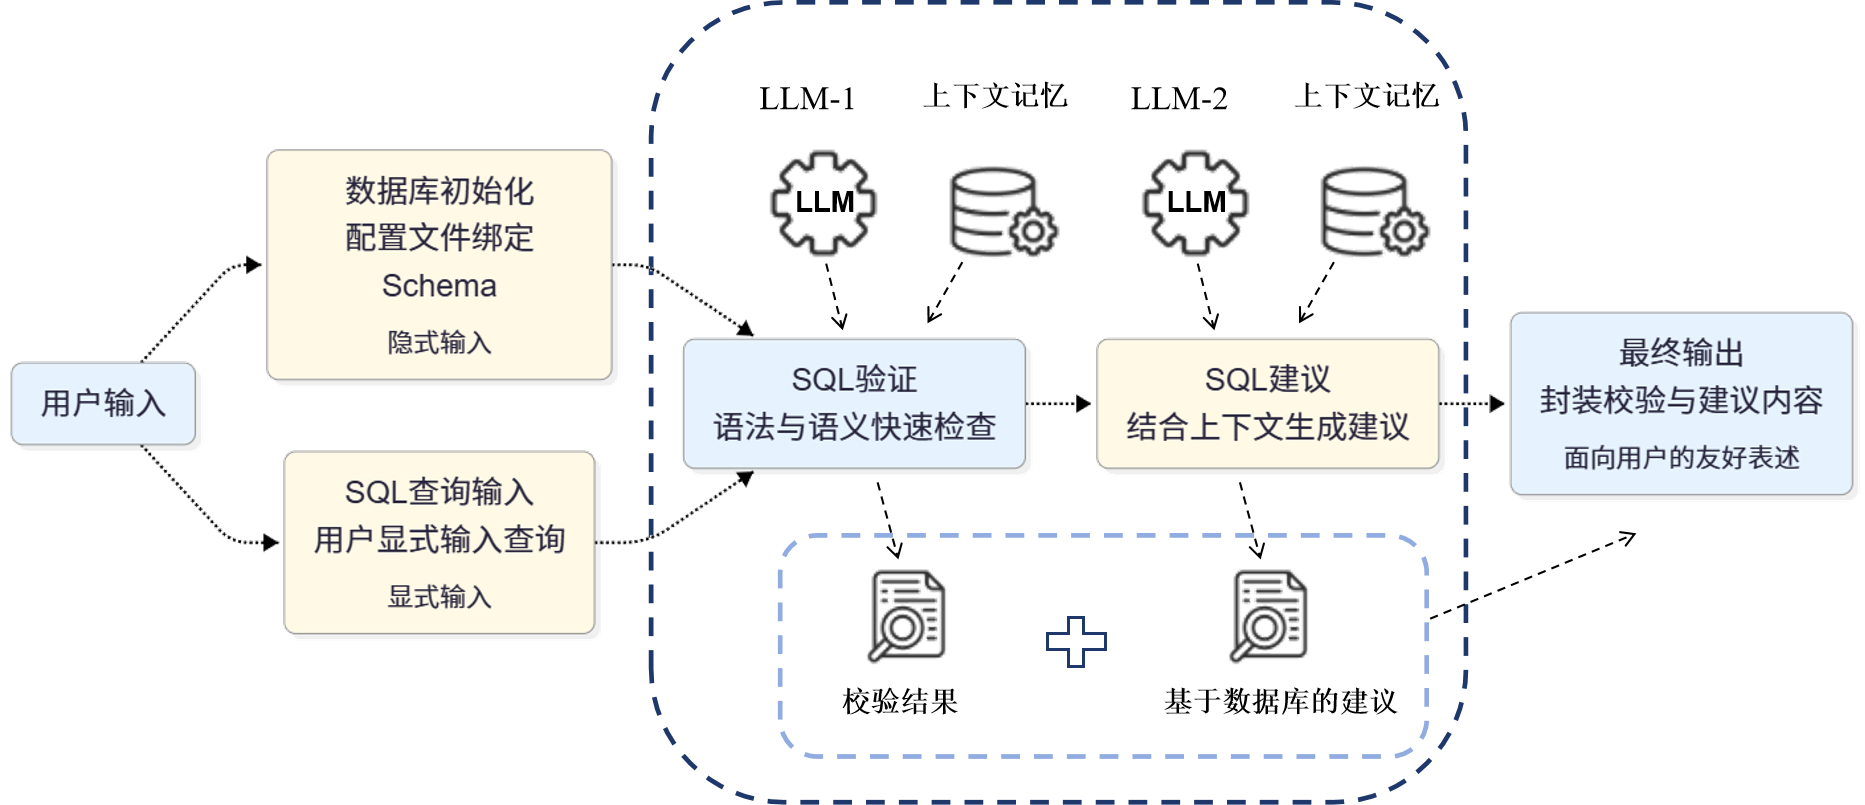
\includegraphics[width=\textwidth]{article/design/figures/workflow}
  \caption{工作流设计}
  \label{fig:agent}

\end{figure*}

Agent的优势在于可以根据实际情况自主规划和执行任务,与任务本身的贴合度高且十分灵活。但为了保证验证过程的可控性与确定性,我们设计了一个简单的工作流来约束SQL验证的主要路径,它同时接受用户的两种输入——显式输入的用户SQL查询,以及隐式加载的数据库Schema,后者在数据库初始化阶段已与配置文件绑定,无需用户再次提供。工作流的最终产出是包含语法语义结构检查、并结合性能与上下文考量的综合结果。其工作流示意图如下。

具体而言,我们注意到SQL验证工具可能存在解释不清、用户不友好问题,因此将SQL验证与SQL建议分为先后的两个任务节点。

SQL验证节点调用用户的SQL输入和数据库schema,执行快速验证,包含语法和语义的检查,返回一个初步的校验结果和对话记忆。SQL建议节点扮演资深数据库工程师与技术导师的角色。它以验证节点的校验结果与诊断上下文为输入,生成具有深度和广度的扩展性建议,运用更贴近工程实践、易于理解的语言,将初步的校验结果与扩展建议重新组织与阐释。最终输出节点将验证和建议的内容总结,打包成完整的验证结果输出。

\textbf{(2)Prompt}

我们的 SQL 验证器遵循简洁高效的提示 (Prompt) 设计策略,并参照工程化的、步骤化的思维链进行设计与部署。我们为智能体设定的角色是“资深SQL及软件工程专家”,角色的任务是接收用户输入,并调用预定义的工作流,对SQL语句进行深度验证,目标是识别并修正语法和语义层面的错误,并提供具有实践价值和用户友好的优化建议,从而全面提升SQL查询的质量。

我们设计了如下三阶段的思维链来拆解SQL验证任务,并将其固化在系统提示词中。

\textbf{1)意图识别与输入解析}

第一阶段负责对用户的原始输入进行标准化处理,以提取出待验证的目标SQL。我们要求该过程遵循以下三条规则:

纯净SQL处理:当输入为不包含任何非SQL字符的纯净SQL语句时,直接将其作为目标输入。

混合输入处理:当输入为自然语言与SQL的混合体时,系统自动提取其中的SQL部分。一个关键的例外是,若自然语言部分包含明确的文本到SQL(Text2SQL)转换意图的指令(例如,“将‘查询所有员工姓名’转换为SQL”),则优先执行转换任务,并将生成的SQL作为目标输入。

输入保真性原则:为保证验证的原始性和准确性,除上述Text2SQL的例外情况外,系统被严格禁止对提取出的SQL进行任何形式的预处理或自动纠错,必须保持其用户输入时的原貌。

\textbf{2)工作流调用与基础验证}

第二阶段是智能体执行分析任务的关键环节,我们要求智能体分三个步骤进行:

工作流启动:将阶段一解析得到的目标SQL语句sql\_input,连同通过配置文件隐式加载的数据库模式db\_info,作为参数调用预设的内部验证工作流。

语义一致性校验:在验证过程中,强制要求对SQL语句中涉及的所有数据库对象与db\_info提供的模式信息进行比对,这是确保语义正确性的关键步骤。

错误诊断与修正生成:若工作流识别出错误,智能体需生成一个或多个修正方案。当存在多种可能性时,模型被要求评估并筛选出最具工程实践价值的几种方案。若未发现错误,则直接确认原始SQL的有效性。

\textbf{3)结果整理与输出}

阶段三将分析结果以一种对用户友好且高度结构化的方式呈现,我们设计了严格的输出格式来约束:

约束性输出格式:最终响应的主体内容是SQL代码。所有的解释、说明、错误提示或优化建议,需要与代码在位置上区分开。

结果呈现逻辑:

① 对于无错误的SQL或仅有单一最优修正建议的场景,输出该条完整的SQL语句。

② 对于存在多个高价值修正建议的场景,则以带编号的列表形式呈现,每条建议后附带其完整的SQL实现,最多展示5种,为用户提供多维度的优化视角。


\end{CJK*}
{\begin{CJK*}{UTF8}{zhhei}\subsubsection{Text2SQL自然语言查询}\end{CJK*}}
\begin{CJK*}{UTF8}{song}

该模块可以将用户的自然语言问题转化为可执行的SQL查询。用户执行 \textit{awesql ask "..."} 时,Text2SQL.get\_schema\_representation() 函数将读取配置文件中记录的 DDL.sql 路径,解析文件内容,并提取所有 CREATE TABLE 语句作为数据库关系模式,用以辅助LLM理解表结构、各个属性的数据类型、是否为主键,外键等。然后,将用户的问题赋值给query变量,关系模式赋值给schema变量,即可以通过填充预定义好的prompt直接输入LLM。此处的LLM为本地部署的sqlcoder-7B,其通过huggingface开源。

最后,LLM将按照prompt模板返回LLM返回包含SQL查询的文本。系统提取出其中的SQL代码块,作为最终的生成结果。此SQL语句随后可以被传递给SQL执行与可视化模块。

\end{CJK*}
{\begin{CJK*}{UTF8}{zhhei}\subsubsection{SQL查询流程与结果可视化}\end{CJK*}}
\begin{CJK*}{UTF8}{song}

此模块负责执行SQL查询并以多种形式呈现其过程与结果。无论是用户直接通过 run命令输入的SQL,还是由 ask命令生成的SQL,都可以被传递到 db.execute\_query() 函数。此函数对输入SQL执行两个操作:1)通过\textit{EXPLAIN QUERY PLAN SQL}: 获取数据库引擎为该查询制定的执行计划;2)通过SQL: 执行查询本身,获取结果数据集。

这两个操作的结果分别被读入两个独立的pandas DataFrame:plan\_df 和 result\_df。其中 plan\_df 被传递给visualizer.draw\_query\_plan ()。该函数将plan\_df重建为树状结构,并匹配预设的解释文案,最后利用 rich 库在控制台渲染出带注释的彩色执行计划树。result\_df 则被用于两种可视化:1)visualizer .print\_results\_table() ,将结果的前10行渲染成一个格式化的控制台表格,供用户快速预览和精确读数。2)visualizer.visualize\_query\_result() ,启动一个交互式会话,引导用户从查询结果的列中选择用于图表 x 轴、y 轴和分类(hue)的数据。根据用户的选择和指定的图表类型(如柱状图、折线图),系统利用 matplotlib 和 seaborn 库生成图表,并将其保存为图像文件,同时自动尝试打开该文件。

为了避免潜在风险,系统会通过正则话自动检测输入的SQL查询,并只允许SELECT查询通过,其他所有与修改和删除相关的命令将被自动禁止并返回警告。

\end{CJK*}
{\begin{CJK*}{UTF8}{zhhei}\subsubsection{系统重置功能}\end{CJK*}}
\begin{CJK*}{UTF8}{song}

此模块用于恢复到初始状态。当用户执行 \textit{awesql reset} 命令,可附带 \textit{--db} 或 \textit{--config} 参数。若指定 \textit{--db},系统调用 db.reset\_db(),该函数通过 os.remove() 直接删除数据库文件;若指定 \textit{--config},系统调用 db.reset\_config(),删除 awesql\_ config.json 配置文件。若无任何参数附加,则默认同时执行上述两个操作。

由于这个操作的破坏性,在CLI层面,执行此命令前会要求用户输入管理员帐号和密码,以防止误操作导致数据丢失。

\end{CJK*}
{\begin{CJK*}{UTF8}{zhhei}\subsubsection{模块连接}\end{CJK*}}
\begin{CJK*}{UTF8}{song}

系统各模块并非孤立存在,而是通过清晰定义的流程和共享的配置进行协作。我们分别展示核心工作流和执行先决条件,以说明系统的工作流程。

核心工作流的命令形式可以展示为$\text{ask} \rightarrow \text{check} \rightarrow \text{run} \rightarrow \text{visualize}$,自然语言查询 (ask) 是起点,其输出(SQL字符串)成为 checker 模块的输入checker.is\_query\_safe() 对SQL进行验证。这一步使用正则表达式和sql-metadata库来禁止如 DROP, DELETE 等危险操作,并检查查询的表和列是否存在于数据库模式中,只有通过检查的SQL才能进入 run 流程,由 db.execute\_query() 执行。当然也可以跳过ask和check命令,直接执行run命令,同样可以在通过检查后执行查询。执行后产生的数据(plan\_df, result\_df)被 visualizer 模块获取并在与用户交互后完成最终的呈现。


 ask, run, er (生成E-R图) 和 check 命令的执行都以一个已初始化的数据库为前提。CLI层在执行这些命令前会检查数据库文件是否存在,若不存在则会中止操作并提示用户先对数据库进行初始化, ask 命令同时依赖 awesql\_config.json 文件来定位 DDL.sql 文件和本地模型路径,er命令则依赖DDL.sql的定位。
 

\end{CJK*}
{\begin{CJK*}{UTF8}{zhhei}\subsubsection{CLI命令}\end{CJK*}}
\begin{CJK*}{UTF8}{song}
\begin{enumerate}
    \item 数据库与环境管理
    
    此类命令负责数据库的生命周期、数据导入以及环境配置。
    \begin{table}[H]
    \centering
    \caption{数据库与环境管理命令}
    \vspace{2mm}
    \small
    \begin{tabular}{p{2cm}p{2cm}p{3cm}}
    \toprule
    \textbf{命令 / 子命令} & \textbf{参数} & \textbf{描述} \\
    \hline
    \texttt{import-data} & \texttt{--dir <PATH>} & 导入数据并创建数据库,基于指定目录的 \texttt{DDL.sql} 和 \texttt{.sql} 文件。 \\
    \texttt{reset-db} & \texttt{--user <TEXT>} & 重置数据库(需管理员权限),删除指定数据库文件。\\
    \texttt{config set-ddl-path} & \texttt{PATH} & 设置 \texttt{DDL.sql} 文件路径,供 Text-to-SQL 功能解析表结构用。 \\
    \texttt{config set-model-path} & \texttt{PATH} & 设置本地 HuggingFace 模型路径,驱动 Text-to-SQL 功能。 \\
    \texttt{config show} & [无] & 显示当前配置,包括模型路径和 DDL 文件路径。 \\
    \bottomrule
    \end{tabular}
    \label{tab1}
    \end{table}

    \item 查询、分析与验证
    
    此类命令是系统的核心功能,用于执行查询、进行AI辅助分析以及保障查询安全。
    \begin{table}[H]
    \centering
    \caption{查询、分析与验证命令}
    \vspace{2mm}
    \small
    \begin{tabular}{lp{2cm}p{3cm}}
    \toprule
    \textbf{命令 / 子命令} & \textbf{参数} & \textbf{描述} \\
    \hline
    \texttt{run} & \texttt{QUERY} (必需) \newline \texttt{--db-name <TEXT>} & 执行SQL查询并可视化结果,包括查询计划和交互式图表。 \\
    \texttt{ask} & \texttt{QUESTION} (必需) & 将自然语言问题转换为SQL查询,并进行安全检查。 \\
    \texttt{check} & \texttt{QUERY} (必需) \newline \texttt{--db-name <TEXT>} & 检查SQL查询的合法性,检测危险操作和语法错误。 \\
    \texttt{tables} & \texttt{--db-name <TEXT>} & 列出指定数据库中的所有表名称。 \\
    \bottomrule
    \end{tabular}
    \label{tab2}
    \end{table}

    \item 可视化与导出
    
    此类命令专注于数据的可视化呈现和导出。
    \begin{table}[H]
    \centering
    \caption{可视化与导出命令}
    \vspace{2mm}
    \small
    \begin{tabular}{p{2cm}p{2cm}p{3cm}}
    \toprule
    \textbf{命令 / 子命令} & \textbf{参数} & \textbf{描述} \\
    \hline
    \texttt{er} & \texttt{--dir <PATH>} \newline \texttt{--output <PATH>} & 生成基于 \texttt{DDL.sql} 的 Mermaid.js E-R 图,输出为 HTML 文件。 \\
    (\texttt{run} 命令的一部分) & (交互式) & 启动交互式图表生成器,允许用户选择图表类型和数据列。 \\
    \bottomrule
    \end{tabular}
    \label{tab3}
    \end{table}

\end{enumerate}
\end{CJK*}

{\begin{CJK*}{UTF8}{zhhei}\zihao{5}\vskip 1mm\section{功能测试与效果展示}\end{CJK*}}

\lstset{
 language=bash,               % 设置语言为bash
 basicstyle=\ttfamily\small,  % 使用等宽字体和较小字号
 keywordstyle=\color{blue}\bfseries, % 关键字样式
 stringstyle=\color{red},     % 字符串样式
 commentstyle=\color{green!50!black}, % 注释样式
 numberstyle=\tiny,          % 行号字体大小
 numbersep=5pt,              % 行号与代码间隔
 showspaces=false,           % 不显示空格
 showstringspaces=false,     % 不强调字符串中的空格
 frame=single,               % 添加边框
 breaklines=true,            % 自动换行
 breakatwhitespace=true,     % 只在空白符处换行
 tabsize=4                   % 制表符宽度
}
\begin{CJK*}{UTF8}{song}

{\begin{CJK*}{UTF8}{zhhei}\subsection{下载与安装}\end{CJK*}}

我们的工具已经开源\footnote{
\url{https://github.com/Hepisces/db_final}}, 接下来将展示使用Anaconda进行包管理下的下载与安装流程。

\begin{figure*}
  \centering
  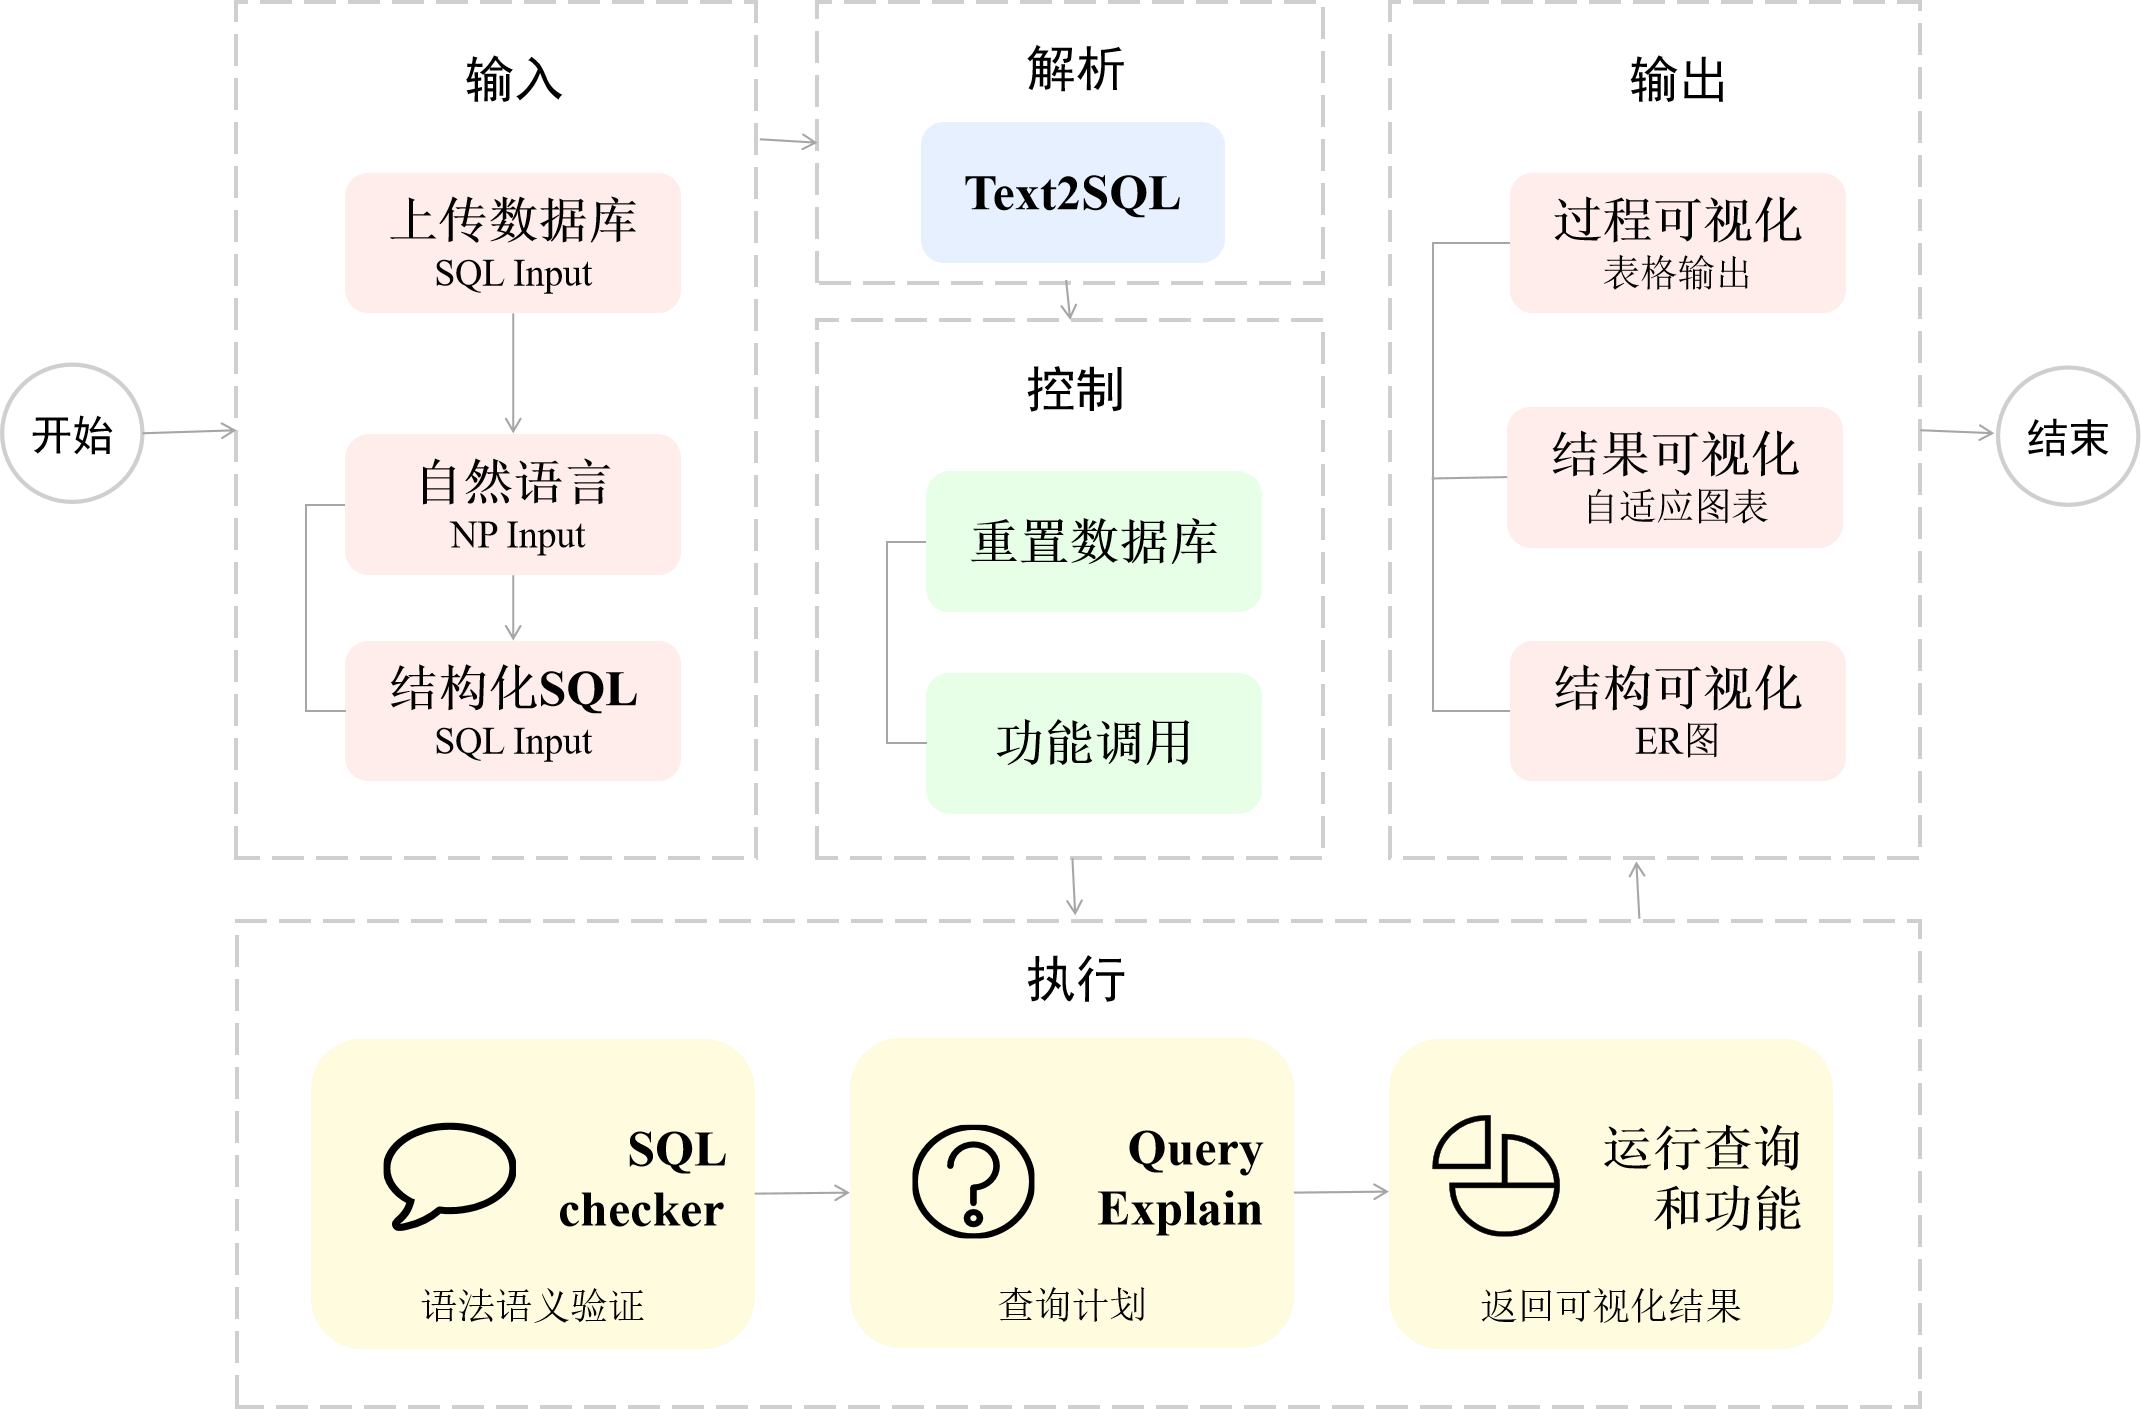
\includegraphics[width=0.9\textwidth]{article/presentation/figures/pipeline}
  \caption{架构设计}
  \label{fig:pipeline}
\end{figure*}

\begin{enumerate}
    \item 首先下载并进入文件夹

\begin{lstlisting}
> git clone \ git@github.com:Hepisces/db_final.git
> cd db_final
\end{lstlisting}

\item 使用conda创建新的虚拟环境
\begin{lstlisting}
> conda create -n awesql python=3.12 -y
> conda activate awesql
\end{lstlisting}

\item 安装相关依赖项,考虑到Text2SQL需要本地模型,下载权重耗时较长,对于简单测试并不是必须的,所以我们提供两种安装方式,当不指定AI选项时,则不会安装Text组件需要的相关库
\begin{lstlisting}
(awesql)> pip install -e .
(awesql)> pip install -e '.[AI]'
\end{lstlisting}
\end{enumerate}

{\begin{CJK*}{UTF8}{zhhei}\subsection{功能测试与效果展示}\end{CJK*}}

为了让展示的效果足够直观,我们为每个命令录制了演示视频,视频可以通过仓库的demo.md文件进行查看。\footnote{
\url{https://github.com/Hepisces/db_final/blob/main/demo.md}}

\begin{enumerate}
    \item 可以通过 help 直接展示各个使用方法

    
    \begin{lstlisting}
(awesql)> awesql --help  
    \end{lstlisting}
    
    \item 导入数据,这里假设你已经下载好了数据并且放到了db\_final的目录下
    \begin{lstlisting}
(awesql)> awesql import-data     
    \end{lstlisting}
    \item 展示当前数据库下的所有表
    \begin{lstlisting}
(awesql)> awesql tables
    \end{lstlisting}
    \item 渲染E-R图
    \begin{lstlisting}
(awesql)> awesql er
    \end{lstlisting}
        \item SQL正确性检查(示例给出的代码错误包括但不仅限于别名错误,非法字符等)
    \begin{lstlisting}
(awesql)> awesql check "SELECT STRFTIME('%Y-%m-%d', d.time) AS date, l.area, COUNT(d.did) AS update.
count, AVG(d.did) FROM devupdata d JOIN devlist | ON d.did = I.did WHERE I.area IS NOT NULL AND
STRETIME('%Y-%m-%d', d.time) > 1999-01-01' GROUP BY date, l.area ORDER BY date;"
    \end{lstlisting}
        \item 通过正确性检查后即可将代码进行查询尝试,后续即可根据交互式命令选择可视化图形类别

    \begin{lstlisting}
(awesql)> awesql run "
SELECT STRFTIME('%Y-%m-%d', d.time) AS date, l.area, COUNT(d.did) AS update_count
FROM devupdata d JOIN devlist l ON d.did = l.did 
WHERE l.area IS NOT NULL AND STRFTIME('%Y-%m-%d', d.time) > '2021-01-01' 
GROUP BY date, l.area ORDER BY date;"        
    \end{lstlisting}
        \item 使用自然语言查询(通常耗时较久,并推荐显存大于24GB的显卡使用)
    \begin{lstlisting}
(awesql)> awesql ask "Querying the time column of the devuplist table"
    \end{lstlisting}
        \item 重置数据库(这一步需要在提示以后输入管理员账户与密码)
    \begin{lstlisting}
(awesql)> awesql reset-db
    \end{lstlisting}
\end{enumerate}



\end{CJK*}
{\begin{CJK*}{UTF8}{zhhei}\zihao{5}\vskip 1mm\section{结论与展望}\end{CJK*}}
\begin{CJK*}{UTF8}{song}

我们围绕SQL语句的验证与分析需求,设计并实现了一款集SQL执行、语句验证、优化建议生成与结果可视化于一体的智能分析工具——Awesql。该工具以命令行交互为核心,面向SQLite数据库环境,构建了从查询输入到图形输出的完整处理链路。通过设计和集成多个智能工具,Awesql显著增强了对SQL查询语义的理解与纠错能力,实现了从静态语法验证到动态语义适配与性能评估的多维升级。

Awesql系统采用高度模块化、可组合的架构设计,不仅便于功能扩展与维护,也兼顾了专业开发人员的控制需求与非专业用户的易用性,在数据库交互智能化、自动化与人机协同方面提供了切实可行的技术路径,是数据库开发工具在智能化方向的一次尝试。具体而言,我们的Awesql在以下方面实现了创新:

(1)端到端的智能分析流程

Awesql打通了从自然语言输入到结构化SQL执行再到数据可视化的完整闭环,构建了统一的交互通道。在架构层面,系统支持SQL语句与自然语言两类输入,并根据任务类型动态调用Text2SQL模块与SQL Checker模块。此外,系统输出不仅包含查询结果,还自动生成符合数据特征的可视化图表,并支持数据库结构的ER图展示,提升了整体数据分析效率与用户认知体验。

(2)智能驱动的模块工具设计与集成

我们构建和接入了Text2SQL工具、基于Agent的SQL checker验证器以及自适应的可视化查询工具。其中SQL checker通过上下文注入与三阶段思维链,系统可在理解用户意图的基础上完成对语法、语义、执行性能及代码规范性的深度分析,最终生成结构化、解释性强的优化建议。

尽管Awesql在功能集成与智能化方面取得了一定成效,但在当前实现中仍存在一些不足。一是当前系统仅适配SQLite数据库,未实现对MySQL、PostgreSQL等主流数据库管理系统及其方言的支持,限制了其在异构数据库环境中的适用性和迁移能力。二是Text2SQL功能依赖于本地部署的大型语言模型,要求较高的计算资源,降低了其在低资源终端或轻量级环境中的可访问性。此外,当前的SQL分析与优化建议主要面向结构较为清晰的查询任务,对于包含嵌套、动态构造或复杂逻辑的SQL语句,系统在语义解析与可视化推荐方面的适应性仍显不足,优化效果与解释能力存在波动。

为进一步增强Awesql系统的适用范围与智能能力,针对这些不足,我们的后续工作将从系统与智能两方面推进:

(1)系统层面

①扩展数据库兼容性:我们希望将当前架构扩展至支持MySQL、PostgreSQL等主流数据库,通过方言适配与执行引擎封装,提升系统的通用性与生态兼容性。


②构建图形化界面或IDE插件:考虑到命令行的使用门槛,我们考虑将Awesql功能封装为VS Code等主流IDE的插件,降低工具的使用难度,拓展用户群体。


③增强可视化交互能力:在现有可视化模块基础上,引入更多可配置参数与图表类型,允许用户进行自定义分析与图形展示,同时支持多维度联动与动态更新。


(2)智能化层面


①Text2SQL优化:结合用户需求与数据库结构,通过更精细的提示工程优化Text2SQL模型,提升在复杂查询中的表现,确保生成的SQL语句更贴合真实需求。

②验证优化:在SQL checker部分,用户输入或查询结果后,系统根据查询的实际执行环,自动选择合适的优化策略,确保生成的SQL语句在不同数据库上都有优异的执行性能。

③一键式操作:现有的Awesql模块支持灵活调用,但考虑工具实际的测试和应用场景,可以加入一键式操作,一次性自动调用Awesql从数据导入到可视化的全流程,降低操作门槛,提高使用便捷性。


\end{CJK*}

    
{\zihao{5}
\begin{CJK*}{UTF8}{zhhei}参~考~文~献\end{CJK*}}
\begin{thebibliography}{99}
\zihao{5-} \addtolength{\itemsep}{-1em}
\vspace {1.5mm}

\bibitem[1]{1}\begin{CJK*}{UTF8}{song}侯博学,陈林 . 数据库技术发展研究综述[J]. 软件导刊,\end{CJK*}
2024,23(6):214-220.
\bibitem[2]{2} \begin{CJK*}{UTF8}{song}宋庆江 . 数据库基础[M]. 西安:西安电子科技大学\end{CJK*}
出版社,2023.
\bibitem[3]{3} Katsogiannis-Meimarakis G, Koutrika G. A survey on deep learning approaches for text-to-SQL[J]. The VLDB Journal, 2023, 32(4): 905-936.


\end{thebibliography}





\end{document}